%%%%%%%%%%%%%%%%%%%%%%%%%%%%%%%%%%%%%%%%%%%%%%%%%%%%%%%%%%%%%%%%%%%%%%%%%%%%%%%%%%%%%%%%%%%%%
%%									Chapitre 3												%
%%%%%%%%%%%%%%%%%%%%%%%%%%%%%%%%%%%%%%%%%%%%%%%%%%%%%%%%%%%%%%%%%%%%%%%%%%%%%%%%%%%%%%%%%%%%%

\chapter{Implémentation de la reconstruction morphologique}
\label{chap:morpho}	
	\minitoc
	

%%%%%%%%%%%%%%%%%%%%%%%%%%%%%%%%%%%%%%%%%%%%%%%%%%%%%%%%%%%%%%%%%%%%%%%%%%%%%%%%%%%%%%%%%%%%%
La reconstruction de la morphologie des vaisseaux est la première étape dans la construction du modèle. Les différentes modalités d’imagerie exposées au chapitre~\ref{chap:imageriemorpho} vont assurer l’extraction quantitative à la fois de l’architecture des vaisseaux et des paramètres géométriques associés : longueurs et aire. \\
Les images d’intérêt issues des différentes modalités d’acquisition doivent être rapportées dans le même espace : les acquisitions en contraste de phase et le $T_1$ sont donc co-registrées (voir Appendice~\ref{sec:pretrait}) avec l’image disposant de la meilleure résolution, l’imagerie par temps de vol. Ce choix permet d’extraire le maximum d’informations. 
%%%
%%%
%%%
\section{Reconstruction du réseau des artères et des veines}
Comme nous l’avons précisé ci-dessus, deux types d’informations doivent être extraites des données structurales : des informations géométriques locales (aire et longueur) mais aussi des informations topologiques sur l’organisation de ce réseau. Le résultat de l’analyse doit donc être de nous fournir un graphe représentant l’arborescence du système. Les deux étapes naturelles sont donc d’abord de segmenter dans nos imageries structurales les parties correspondantes au système circulant puis d’extraire la topologie de ce système. Cet objectif impose des contraintes spécifiques, telles que l’intégrité et la complétude du réseau qui gouverne les choix fait dans les étapes successives.\\
L’un des critères importants à prendre en compte lors de la sélection de la chaîne de traitement est le degré d’implication de l’utilisateur. A quels moments et combien de fois doit il intervenir ? Pour nous, l’idéal serait de réduire au maximum cette intervention, ou du moins de la limiter à des actions simples. 
%%%
%%%
\subsection{Segmentation}
Que ce soit en imagerie par temps de vol ou en contraste de phase, les vaisseaux (artères et veines) apparaissent avec une intensité plus élevée que les autres tissus. L’approche la plus simple est donc de seuiller l’image afin d’en extraire les hypersignaux, et donc les vaisseaux. Cette approche permet de récupérer rapidement une segmentation mais le résultat reste très sensible aux inhomogénéités du signal et au bruit, qui peuvent en diminuer la qualité (Figure~\ref{fig:2_1_segmentation_arteres}).\\
\begin{figure}[!t]
\centering
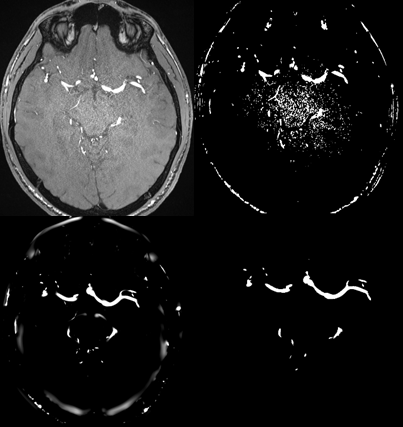
\includegraphics[width=9cm]{2_1_segmentation_arteres}
\caption{Illustration de la segmentation des artères à partir d’une image de temps de vol. A) Image ToF brute, B) Image seuillée manuellement, C) Image filtrée par le filtre de Frangi, D) Image filtrée seuillée.}
\label{fig:2_1_segmentation_arteres}	
\end{figure}
Un grand nombre d’outils de segmentation existent dédiés aux images IRM. Mais ils recherchent un but spécifique : l’extraction des différents types de tissus présents dans le cerveau, la matière grise, la matière blanche, et le liquide cérébro-spinal (voir Appendice~\ref{sec:pretrait}).  Les approches optimisées pour ce genre de segmentation ne peuvent pas être appliquées dans le cadre des vaisseaux. Pour ces derniers des approches dédiées ont été développées (\cite{Lesage2009}). Elles se décomposent toutes en deux étapes, chacune devant être optimisée : le prétraitement des images puis la segmentation elle-même.\\
Les prétraitements consistent à simplifier les informations contenues dans les images d’angiographie IRM. Les traitements génériques disponibles entre lesquels il s’agît de faire un choix ont été développés dans d’autres contextes comme le sous-échantillonnage et la quantification (\cite{Tschirren2005}). Les outils les plus courants restent cependant les filtres améliorant la qualité de l’image. Citons les filtres gradients  (\cite{Koller1995}), les filtres morphologiques (\cite{Wilkinson2001}), ou les filtres à base de matrice Hessienne (\cite{Frangi1998}). \\
A l’issue du prétraitement, les principaux algorithmes de segmentation utilisés dans des contextes vasculaires se regroupent en trois approches principales : la croissance de région, les contours actifs, et les lignes médianes (\cite{Lesage2009}). La croissance de région segmente de façon incrémentielle un objet en recrutant les voxels adjacents selon certains critères comme par exemple la variation locale de l’intensité. Elle requiert le plus souvent la définition d’un point initial, qui peut être obtenu via un simple seuillage sur l’image (\cite{Boskamp2004}). Les contours actifs font évoluer une interface sous l’action de différentes forces : des forces externes calculées à partir des intensités de l’image, et des forces internes de type tension de lignes exprimant des contraintes a-priori la géométrie du contour et sa régularité (\cite{McInerney1996}). Les lignes médianes se focalisent sur l’extraction directe du centre des vaisseaux en utilisant des informations de plus haut niveaux telles que la localisation du centre du vaisseau, l’estimation de sa direction et de sa taille caractéristique (\cite{Aylward2002}).\\
%%%
\begin{figure}[!t]
\centering
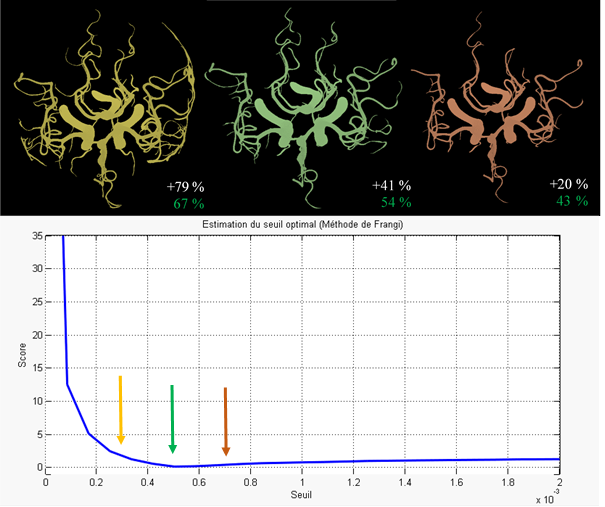
\includegraphics[width=12cm]{2_optimisation_criteres}
\caption{Estimation du seuil optimal selon un critère qualité. La méthode de segmentation illustrée est le seuillage après filtre de Frangi. La courbe montre l'évolution du score en fonction du seuil. Par soucis de clarté le score est convertie de telle sorte à ce que le proche de zéro corresponde au paramètre optimal. Le score prend en compte la correspondance avec un squelette d'une segmentation de référence (manuelle) et sur l'écart en termes de volume entre la référence et la segmentation donnée pour les 100 premiers niveaux de coupes (zone la plus facilement segmentable). La valeur indiquée par la flèche verte est l'optimale, la jaune légèrement en dessous et l'orange au dessus. Les segmentations correspondantes sont illustrées avec les couleurs associées. En vert est indiqué le pourcentage de recouvrement de la segmentation donnée en rapport de la référence et en blanc l'écart de volume en pourcent avec la référence. Notons que pour chaque segmentation, seul les plus grosses structures sont retenues}
\label{fig:2_optimisation_criteres}	
\end{figure}
%%
%%%
\begin{figure}[!t]
\centering
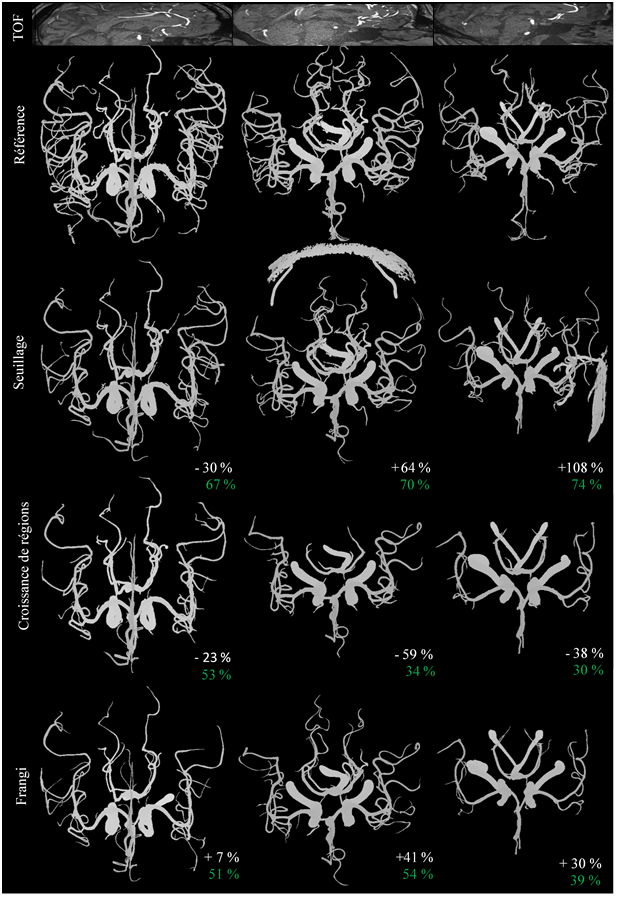
\includegraphics[width=15cm]{2_comparaisons_segmentations}
\caption{Comparaison de différents algorithmes de segmentation sur 3 images par temps de vol de couverture anatomique différentes. Une segmentation manuelle a été réalisée et validé par un neuroradiologue afin de servir de référence. Trois méthodes de segmentations sont ici comparées : seuillage sur l'intensité, croissance de régions et filtre de Frangi. Pour chaque méthode les paramètres ont été ajustés automatiquement. En première ligne est affichée une vue sagittale du volume. En vert est indiqué le pourcentage de recouvrement de la segmentation donnée en rapport de la référence et en blanc l'écart de volume en pourcent avec la référence. Notons que pour chaque segmentation, seul les plus grosses structures sont retenues.}
\label{fig:2_comparaisons_segmentations}	
\end{figure}
%%
Afin d'évaluer la pertinence des principales segmentations, nous avons appliqué sur trois images TOF de couvertures anatomiques différentes, différents algorithmes  (Figure~\ref{fig:2_comparaisons_segmentations}). Nous avons ainsi testé le seuillage simple, la croissance de région et le seuillage sur la base d'un filtre de Frangi (prétraitement Hessien). Pour chaque volume TOF, une segmentation manuelle validée par un neuroradiologue a été réalisée pour de servir de référence. Son squelette a ensuite été extrait par amincissement itératif (voir ~\ref{ss:skel}). Notons d'ailleurs que parmi les trois volumes, le premier possède une couverture anatomique proche des données BraVa. Les longueurs des différentes artères sont d'ailleurs en accord avec cette base (voir Table~\ref{tab:databrava}). Chaque méthode requiert l'ajustement de paramètres permettant l'obtention d'une segmentation de bonne qualité. En vue de les optimiser, nous avons établit un score prenant en compte 1) le pourcentage du squelette de référence inclus dans la segmentation, et 2) le rapport moyen entre le volume de la segmentation donnée et de la référence pour les 100 premiers niveaux de coupes (où les vaisseaux sont le plus facilement segmentable). Les paramètres de segmentation sont définis comme optimaux lorsque le score est proche de 2 (somme des deux critères). Un exemple d'identification de ces paramètres est donné en Figure~\ref{fig:2_optimisation_criteres} sur un seuillage après filtre de Frangi.  Comme on le voit, un seuil plus faible que l'optimal permet de récupérer une plus grande partie de l'arbre artériel (67\%) mais avec une surestimation de son volume de l'ordre de 79\%. Une valeur supérieure induit au contraire une perte d'une partie de l'arborescence (43 \%) mais affine le volume (+20\% seulement d'écart avec la référence). Le paramètre optimal assure un compromis entre couverture de l'arbre vasculaire (54\%) et volume (+41\%). On notera ainsi que méthode de Frangi à tendance à surestimer le volume artériel.\\

 Les segmentations obtenues par les différentes méthodes après utilisation de ce critère qualité sont illustrées dans la Figure~\ref{fig:2_comparaisons_segmentations}. Le simple seuillage semble offrir la meilleur correspondance en terme de recouvrement de l'aborescence totale pour les trois volumes avec une moyenne de 70\%, en revanche des écarts important en termes de volume peuvent être identifiés. Ceux-ci sont principalement dûs à la segmentation d'autres structures ou de bruit identifié comme du vaisseau à cause des inhomogénéités de signal. Ce phénomène se voit clairement sur les deux derniers volumes. La croissance de région quant à elle offre des résultats mitigés avec seulement 39\% de recouvrement et une sous estimation systématique du volume (40\%). Cette sous estimation s'explique par le fait que l'algorithme requiert des points initiaux pour développer la segmentation. Selon leur localisation, la méthode segmentera plutot la périphérie du vaisseau ou son centre induisant donc une sous estimation du volume. Le seuillage d'un filtre de Frangi (prétraitement Hessien), permet de récupérer 48\%  de l'arbre vasculaire en moyenne avec une certaine constance. Contrairement au seuillage simple, il ne récupère que les vaisseaux et non le bruit. Le volume est cependant systématiquement sur-estimé. Notons que nous avons par ailleurs réalisé des essais avec un algorithme de contour actif (non illustrés ici), ceux ci mettent en évidence un temps de traitement bien plus long (en heure contre quelques minutes pour les autres) pour un résultat proche de la croissance de région: sous estimation du volume de l'ordre de 24\% et 41\% de couverture de l'arbre vasculaire pour le premier volume.\\

Au vue des résultats nous avons choisi la combinaison d’un prétraitement Hessien suivit d’un seuillage simple qui, malgré un recouvrement plus faible de l'arbre vasculaire en comparaison du seuillage simple, assure une identification des vaisseaux uniquement. Le filtre Hessien est en effet robuste dans sa capacité à fournir une image très contrastée des vaisseaux, à partir de laquelle un simple seuillage ajusté manuellement (intervention de l’utilisateur) fournit un résultat qui rend superflu l’utilisation de méthodes de segmentation plus sophistiquées. \\
Le filtre utilisant cette méthode est dit filtre de Frangi  (\cite{Frangi1998},~\cite{Manniesing2006}). Ce filtre vise à extraire une quantité mesurant la vraisemblance pour une région d’appartenir à un vaisseau : on parle de  « vesselness » locale de l’image. L’idée est d’identifier dans l’image les structures en forme de tubes (voir Figure~\ref{fig:2_1_segmentation_arteres}).\\
%%%
\begin{figure}[!t]
\centering
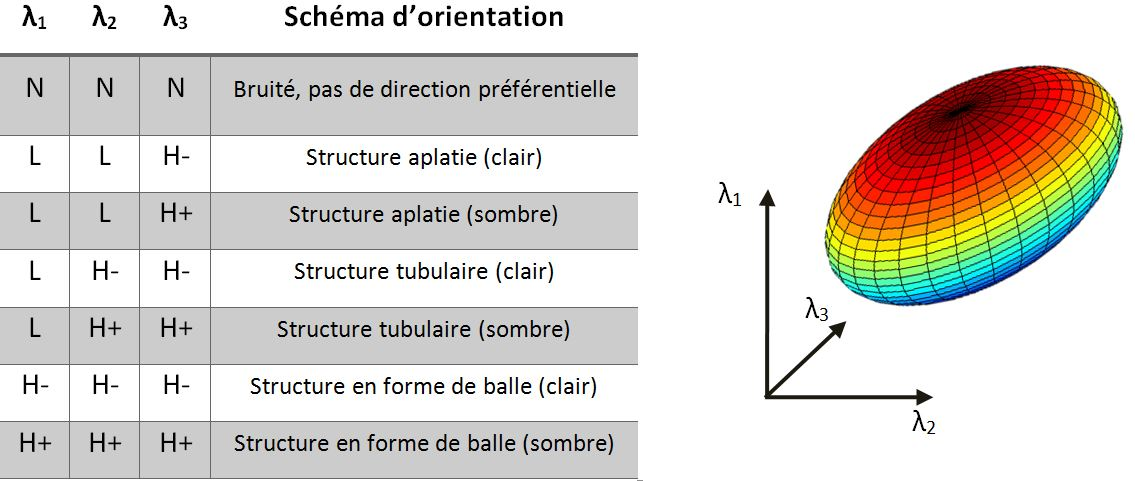
\includegraphics[width=15cm]{2_2_tableau_hessienne}
\caption{Schéma possible en 3D selon la valeur de la valeur propre $\lambda_k$ (H=élevé, L=faible, N = bruité, +/- indique le signe de la valeur propre). Les valeurs propres sont ordonnées selon ($|\lambda_1|\leqslant |\lambda_2|\leqslant |\lambda_3|$ (\cite{Frangi1998}).}
\label{fig:2_2_tableau_hessienne}	
\end{figure}
Mathématiquement, on calcule la matrice Hessienne de l’image à partir de ses dérivées secondes (aux différences finies) et on en extrait des valeurs propres. Ces valeurs propres $\lambda_1$, $\lambda_2$ et $\lambda_3$ (à 3D) caractérisent l’anisotropie des intensités de l’image. Les valeurs propres sont classées par ordre croissant du module ($|\lambda_1|\leqslant|\lambda_2|\leqslant|\lambda_3|$). Un voxel appartenant à un vaisseau doit se caractériser par un ellipsoïde Hessien local allongé : $\lambda_1$ faible (idéalement zéro) et $\lambda_2$ et $\lambda_3$ de grandes magnitudes de mêmes signes. Le tableau de la figure~\ref{fig:2_2_tableau_hessienne} résume les relations existantes entre les valeurs propres de la matrice Hessienne et les différentes structures que l’on cherche à détecter. Avec l’imagerie ToF et le contraste de phase, nous recherchons ainsi les structures claires tubulaires. Le résultat de cette étape est une image dont les intensités représentent pour chaque pixel la vraisemblance d’appartenance à un vaisseau (Figure ~\ref{fig:2_1_segmentation_arteres} C). L’image filtrée est de très bonne qualité (Figure~\ref{fig:2_3_filtre_frangi}). L’utilisation de cet outil moins sensible au bruit et offrant des contours plus lisses, facilite donc les étapes postérieures de traitement. Un simple seuillage, ajusté manuellement, suffit à extraire le volume 3D des vaisseaux (Figure ~\ref{fig:2_1_segmentation_arteres} D, Figure \ref{fig:2_4_segemtation_cont_phase_tof}). Nous n’avons pas besoin de d’utiliser des algorithmes de croissance de région ou autre. L’utilisateur n’a qu’à adapter le seuil, pour extraire les voxels du masque appartenant aux vaisseaux. 
%%%
\begin{figure}[!t]
\centering
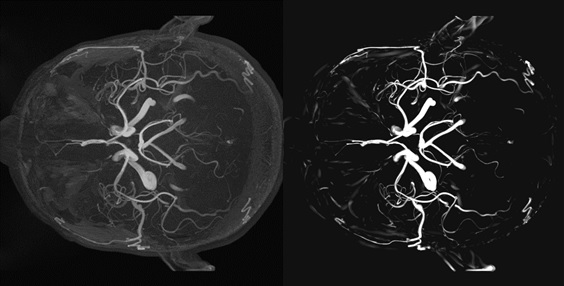
\includegraphics[width=13cm]{2_3_filtre_frangi}
\caption{Comparaison entre une projection des intensités maximales sur une image en temps de vol brute à gauche, et l'image filtrée par le filtre de Frangi à droite. L'image filtrée est moins bruitée et met en évidence les vaisseaux d'intérêt.}
\label{fig:2_3_filtre_frangi}	
\end{figure}	

%%%
\begin{figure}[!b]
\centering
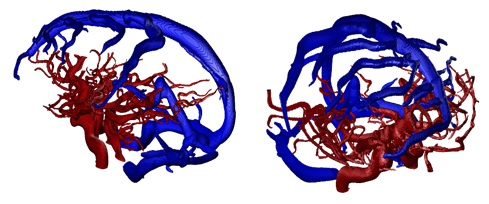
\includegraphics[width=13cm]{2_4_segemtation_cont_phase_tof}
\caption{Segmentations 3D obtenues à partir du contraste de phase (veines, bleu) et du ToF (artères, rouge).}
\label{fig:2_4_segemtation_cont_phase_tof}	
\end{figure}	

Comme on l’a vue dans le chapitre précédent, les images par temps de vol fournissent une information artérielle. Le contraste de phase par contre met en évidence à la fois le versant veineux et artériel. Pour segmenter les veines, l’information artérielle doit donc être éliminée des images du contraste de phase. Il est donc indispensable de segmenter en premier lieu l’imagerie par temps de vol, d’identifier les artères, et de les soustraire de l’image en contraste de phase. La même méthodologie (filtre de Frangi et seuillage) sera ensuite appliquée sur cette image. En effet, les résultats sur cette imagerie sont similaires à ceux exposés dans la Figure~\ref{fig:2_comparaisons_segmentations}. Notons cependant que la croissance de région s'avère plus compliquée du fait de l'inhomogénéité du signal dans les différents types de vaisseaux.\\

Les volumes 3D obtenus (Figure \ref{fig:2_4_segemtation_cont_phase_tof}) reflètent l’arborescence veineuse et artérielle et fournissent une base solide l’extraction des données géométriques et topologiques. De plus, l’apport de la carte de susceptibilité magnétique se fait ressentir principalement au niveau des petites veines (Figure~\ref{fig:2_5_segmentation_apport_QSM}).
%%%
\begin{figure}[!t]
\centering
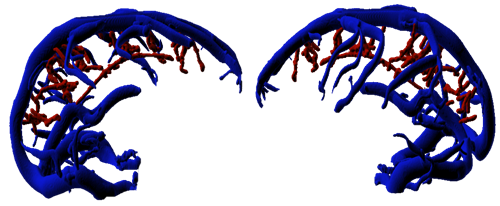
\includegraphics[width=13cm]{2_5_segmentation_apport_QSM}
\caption{Illustration de l'apport de l'information de la QSM dans la définition de l'arborescence veineuse. En bleu les veines identifiées en contraste de phase et en rouges celles issues de la QSM.}
\label{fig:2_5_segmentation_apport_QSM}	
\end{figure}	
%%%
%%%
\subsection{Extraction du squelette}	
\label{ss:skel}
La segmentation permet d’aboutir à un volume 3D représentant notre arbre vasculaire. Cependant en l’état il ne renseigne pas sur la structure du réseau. Pour identifier les différents segments et points de jonction, et réduire la quantité de données, il est indispensable d’extraire le squelette du masque et de le représenter sous forme de graphe. \\

Le squelette est une représentation très utilisée car il contient et résume les propriétés topologiques de la forme qu’il représente. Il permet  de décrire les objets par un ensemble de lignes fines réduisant sensiblement le volume d’informations à manipuler. Le squelette est généralement défini comme étant l’ensemble des lignes médianes, c’est-à-dire l’ensemble des points équidistants de deux points de la frontière. Notons que sa construction est très sensible à la qualité de la segmentation, en particulier au bruit.  \\

Il existe une grande variété de méthodes permettant de construire des squelettes à partir de formes données. La plus commune est la méthode dite d’extraction de la carte des distances, qui consiste à calculer en chaque point interne à l’objet, la distance à son contour le plus proche. Une fois cela réalisé, les maximums locaux de cette carte sont récupérés et forment le squelette de l’objet (Figure~\ref{fig:2_6_squelettisation}). 
%%%
\begin{figure}[!b]
\centering
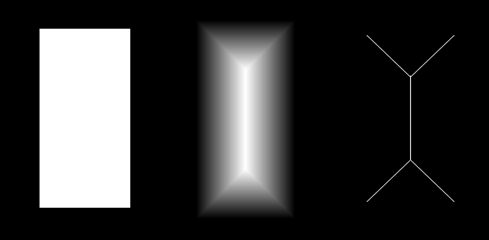
\includegraphics[width=13cm]{2_6_squelettisation}
\caption{Création du squelette d'un rectangle par utilisation de la carte des distances. De gauche à droite, le rectangle brut, la carte de distance, et le squelette.}
\label{fig:2_6_squelettisation}	
\end{figure}	

De façon similaire à la méthode des cartes de distances, la méthode des potentiels généralisés génère un champ à l’intérieur de l’objet. Ce champ n’est plus une simple distance mais un potentiel de type Newtonien, déterminé comme la somme des potentiels gravitationnels générés par des masses placées sur les limites de l’objet. Ce type de méthode peut trouver un grand nombre de variantes en changeant la définition du champ scalaire calculé pour les points intérieur du masque et dont on cherche l’extremum. \\

Enfin, la méthode dite d’amincissement itératif consiste à retirer au fur et à mesure les points du contour de la forme par érosion (\cite{Palagyi2002}), tout en préservant ses caractéristiques topologique. Dans cette approche l’axe médian de l’objet est identifié. Les voxels sont itérativement éliminés de la surface du volume si leur suppression n’affecte pas la connectivité de leur voisinage de 3 x 3 x 3, et si ils ont plus d’un voisin dans ce voisinage. Sinon ils sont définis comme des points terminaux. L’érosion doit être réalisée de façon symétrique afin de garantir la position médiane des lignes du squelette.\\

Il existe deux approches majeures dans les méthodes d’amincissement itératif : les filtres et  les arbres de décisions. Les filtres appliquent un élément structurant à l’image et peuvent généralement être étendus à des dimensions supérieures à 3D  (\cite{Jonker2000}). Les méthodes basées sur des arbres de décision sont limitées à des données 2D et 3D, mais sont plus rapides que les filtres morphologiques. \\
Un algorithme de ce type (\cite{Lee1994}) repose sur un processus itératif dans lequel chaque pixel est testé afin de savoir s’il peut être érodé de l’objet. Le pixel peut être supprimé : 
\begin{itemize}
\item S’il est un pixel de surface. Ce test ne considère qu’une des six directions possible en 3D (Nord, Sud, Est, Ouest, Dessus, Dessous) à la fois afin de réaliser l’amincissement de façon symétrique;
\item S’il n’est pas la fin d’une ligne;
\item Si la suppression du point ne change pas la caractéristique d’Euler, par exemple si aucun trou n’est créé lorsque le pixel est retiré (voir table d’Euler de~\cite{Lee1994});
\item Si le point est un point simple, c’est-à-dire qu’il que sa suppression ne change pas le nombre d’objets connectés.
\end{itemize}
Ce processus est réalisé en parallèle pour chaque pixel de l’image, et répété jusqu’à ce qu’il n’y ait plus de changements. Lee et al. (~\cite{Lee1994}) ont démontré dans leurs travaux, que leur solution basée sur un arbre de décision est capable de trouver correctement l’ensemble des points supprimables à chaque itération. Leur algorithme d’érosion est très rapide.\\

Les résultats obtenus via les différentes approches sont visible sur la Figure~\ref{fig:2_7_skeleton_matlab_toolbox}. 
%%%
\begin{figure}[!t]
\centering
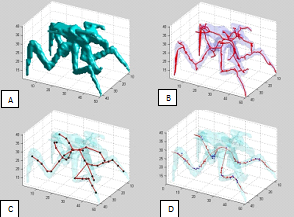
\includegraphics[width=13cm]{2_7_skeleton_matlab_toolbox}
\caption{Exemple de génération de squelette à partir d'un objet avec différentes méthodes. A) Objet brut, B) Squelette par amincissement itératif, C) squelette par carte des distances et D) squelette par carte de champ potentiels. Figure générée par utilisation de la toolbox {\tt Volume Skeleton Matlab Toolbox} (Liu, Rutgers University).}
\label{fig:2_7_skeleton_matlab_toolbox}	
\end{figure}	
Comme on le voit ces différentes approches fournissent différents niveaux de détails sur la structure d’intérêt. Il est donc nécessaire d’évaluer au vu de l’objectif quel niveau de détails nous souhaitons atteindre. Dans notre travail, nous devons extraire le squelette de vaisseaux de diamètres extrêmement variables, et parfois très tortueux. Après quelques tests nous avons décidé d’utiliser la méthode d’amincissement itératif décrit par Lee (\cite{Lee1994} voir Figure~\ref{fig:2_7_skeleton_matlab_toolbox} B) via l’implémentation Matlab fournit par Kerschnitzki et associés (\cite{Kerschnitzki2013}).\\

L’utilisation de cet algorithme sur notre segmentation aboutit à une structure reflétant relativement bien notre topologie initiale (Figure~\ref{fig:2_8_structure_extraite}).
%%%
\begin{figure}[!t]
\centering
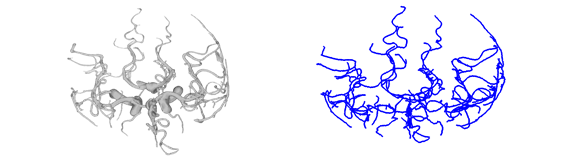
\includegraphics[width=13cm]{2_8_structure_extraite}
\caption{Application de la méthode d'amincissement itératif à une segmentation artérielle. A gauche la segmentation et à droite le squelette résultant. Le résultat est similaire avec les veines.}
\label{fig:2_8_structure_extraite}	
\end{figure}	
%%%
%%%
\subsection{Création du graphe}
\label{sect:graph_creation}
L’arbre vasculaire contient de nombreux vaisseaux qui se subdivisent ou se rejoignent,  par exemple au niveau du polygone de Willis. Les structures les plus adaptées pour la représentation de la topologie de ces architectures complexes sont les graphes et plus précisément les graphes orientés. En théorie des graphes, un graphe orienté est défini par un ensemble de nœuds (ou sommets) reliés par des arrêtes (ou liens) orientées. Dans le réseau, un nœud pointe vers un autre dans une direction spécifique. Dans notre contexte les liens représentent les segments de vaisseaux et les nœuds les jonctions entre ces vaisseaux. Notons que la description admet des liens « terminaux » appelés branches qui ne se terminent pas eux même par un nœud (Figure~\ref{fig:2_9_branches_noeuds}).\\
%%%
\begin{figure}[!t]
\centering
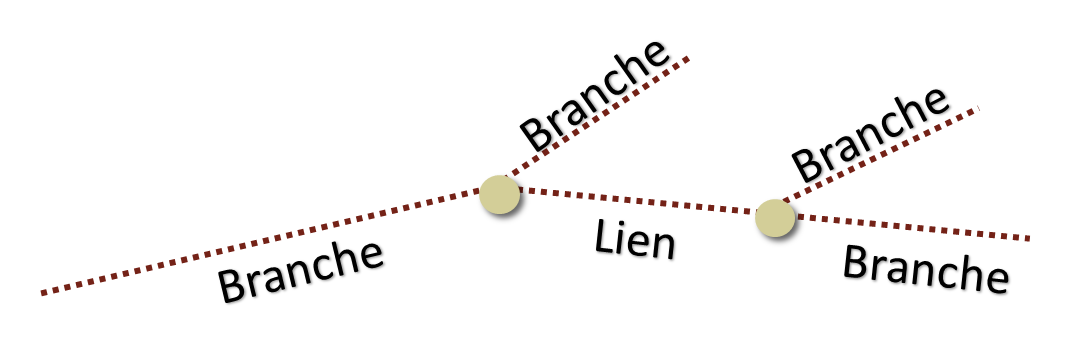
\includegraphics[width=16cm]{2_9_branches_noeuds}
\caption{Illustration d'un graphe, les cercles représentent les nœuds.}
\label{fig:2_9_branches_noeuds}	
\end{figure}	

Le passage d’un squelette à une structure de graphe peut être réalisé simplement. On définit comme nœud les groupes de voxels disposants de plus de deux voisins chacun. Les groupes de voxels possédants exactement deux voisins appartiennent à des liens ou à des branches si ils ne se connectent qu’à un nœud (\cite{Kerschnitzki2013}). Cette conversion est standard : nous avons utilisé l’implémentation de Kollmannsberger(\cite{Kerschnitzki2013}). \\

Le passage de la segmentation brute au squelette puis au graphe conduit à l’apparition d’erreurs telles que la création de faux liens de faibles longueurs ou de fausses anastomoses (Figure~\ref{fig:2_10_boucles}). Il convient donc de les détecter et de les retirer. C’est ce que nous avons mis en place.
%%%
\begin{figure}[!b]
\centering
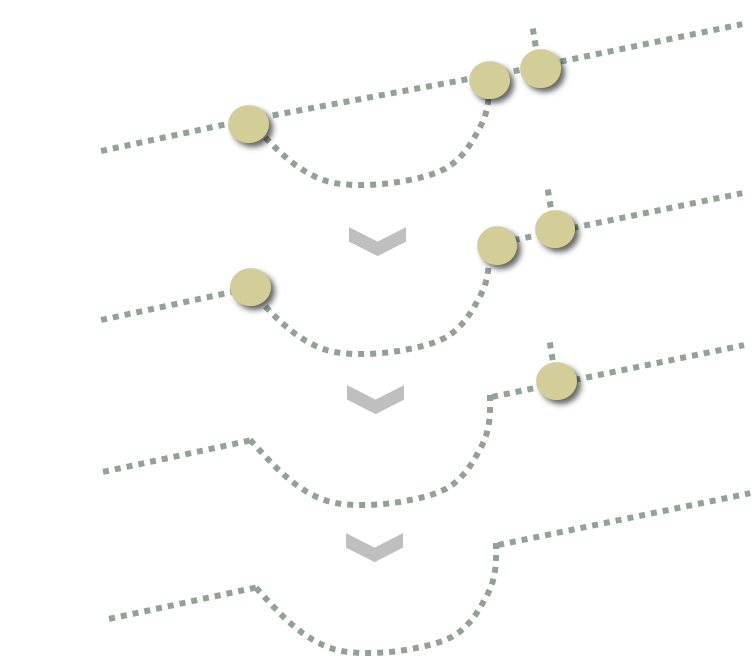
\includegraphics[width=7cm]{2_10_boucles}
\caption{Illustration de l'élimination automatique des erreurs mis en place. De haut en bas l’évolution du graphe, avec élimination des doubles liens directs, des nœuds en série, puis des segments courts.}
\label{fig:2_10_boucles}	
\end{figure}	
On repère tout d’abord les nœuds ayant un double lien direct avec un autre nœud (une distance maximale est utilisée) et on ne conserve que le lien le plus long. On élimine ensuite les nœuds en série de telle sorte à ce que l’on n’ait pas de sous segments pour un même vaisseau. On identifie et supprime les branches les plus courtes (< 2 mm). On réitère ce processus jusqu’à nettoyage complet du graphe. Le résultat est représenté dans la Figure~\ref{fig:2_11_nettoyage_graphe}.\\
%%%
\begin{figure}[!t]
\centering
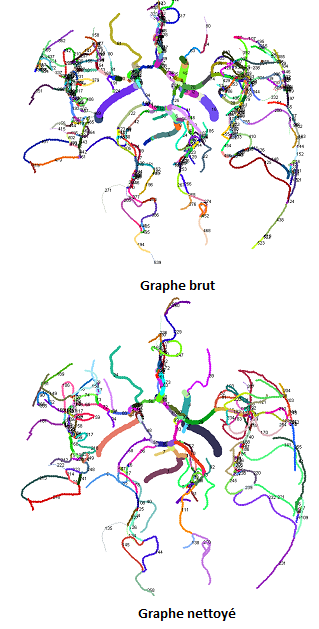
\includegraphics[width=10cm]{2_11_nettoyage_graphe}
\caption{Exemple de nettoyage automatique d'un graphe artériel. En haut le graphe brut, en bas le graphe nettoyé.}
\label{fig:2_11_nettoyage_graphe}	
\end{figure}	

Cette méthodologie assure une cohérence à la description topologique fournie par le graphe final (Figure~\ref{fig:2_11_nettoyage_graphe}). Notons malgré tout qu’une étape manuelle est indispensable. Au niveau artériel, on demande à l’opérateur 1) de cliquer sur les liens qui lui paraissent complètement incohérents et 2) d’indiquer si la séparation entre les deux artères cérébrales antérieures n’est pas bonne, de manière à dupliquer les segments (un par hémisphère), la segmentation ayant souvent du mal à les séparer.\\

Par ailleurs la construction automatique ultérieure des équations du modèle demandera de re-parcourir ce graphe en disposant d’informations supplémentaires que l’opérateur doit également fournir à ce stade. Au niveau artériel l’utilisateur doit 1) cliquer sur les artères communicantes, s’il y en a, pour les identifier, et 2) indiquer au niveau des principales intersections, les hémisphères (cette information sera propagée dans le reste de l’architecture de proche en proche). Au niveau veineux on demande à l’utilisateur l’identification de l’hémisphère pour les veines latérales.\\

Pour chaque segment il est enfin nécessaire d’extraire les caractéristiques géométriques : volumes, diamètres et longueurs afin de les caractériser et les décrire. Pour ce faire, nous employons une approche simple qui associe à chaque voxel de la segmentation un label qui le lie au segment le plus proche du squelette en termes de distance euclidienne. On aboutit ainsi à une labélisation en segments du masque des vaisseaux, on récupère ensuite le volume de chaque segment auquel on associe également une longueur identifiée par le nombre de voxels du segment correspondant du squelette. On peut ensuite extraire le rayon en considérant la structure curviligne comme étant de section constante via
\begin{equation}
\label{eq:rayons}
Rayon\,=\,\frac{Volume}{Longueur\,\pi},
\end{equation}
où l’on a négligé les écarts de volumes entre tube curviligne et tube droit. 
%%%
%%%
%%%
\section{Artérioles – capillaires - veinules}
Les informations artérielles et veineuses peuvent être récupérées par IRM. En revanche les données morphologiques sur les artérioles, capillaires et veinules ne sont pas atteignables à la résolution disponible. Ces compartiments représentent une véritable boite noire pour laquelle il est indispensable de faire des hypothèses basées sur la littérature afin de les représenter au mieux dans le modèle.
%%%
%%%
\subsection{Quelle artère avec quelle veine ? }
Dans une première étape nous devons associer une artère et une veine comme cela se produit physiologiquement, l’ensemble constitue un territoire artério-veineux. Il existe une très forte variabilité de ces territoires du côté veineux en particulier (\cite{Reiner2013}). L’information que l’on pourrait souhaiter utiliser serait un atlas des territoires veineux mais cette variabilité rend impossible l'association fine d'une artère à une veine.\\

En l’état de l’imagerie nous avons sélectionné une approche simple consistant à trouver la veine la plus proche de l’extrémité de chaque branche du système artériel, en utilisant une distance euclidienne. Si ensuite une veine n’est toujours pas reliée à une artère, l’artère la plus proche est réciproquement recherchée et associée à cette veine (Figure~\ref{fig:2_12_liens_arteres_veines}).
%%%
\begin{figure}[!t]
\centering
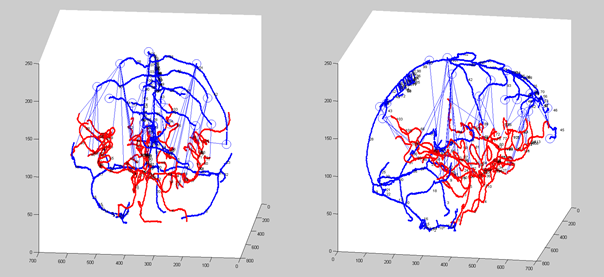
\includegraphics[width=14cm]{2_12_liens_arteres_veines}
\caption{Illustration des liens effectués entre les artères et les veines. Les cercles bleus représentent les extrémités des branches et les lignes bleues fines les liaisons.}
\label{fig:2_12_liens_arteres_veines}	
\end{figure}	
%%%
%%%
\subsection{Estimation des paramètres des tubes}
\label{sec:tubesestimates}
La distance euclidienne entre artère et veine permet de proposer une longueur totale approchée, qui correspondra à la somme des artérioles, capillaires et veinules.  Nous n’avons aucun moyen d’accéder directement aux informations morphologiques de ces compartiments. Pour limiter le nombre d’hypothèses à réaliser sur le nombre de vaisseaux, il semble plus logique de ne considérer pour chaque couple artère-veine qu’une « super-artériole », qu’un « super-capillaire », et qu’une « super-veinule » regroupant un ensemble N de vaisseaux. Bien que ces compartiments soient difficilement accessible (voir~\ref{sect:microcirculation}), la littérature nous fournit quelques informations sur les rapports de ces différents compartiments via des volumes moyens (\cite{Zagzoule1986}, \cite{Linninger2009}). Parmi celles-ci on retrouve des rapports de longueurs et de volumes. Par ailleurs~\cite{Moody2004} ont estimé la fraction de volume que représentent les artérioles et les capillaires dans la matière grise et blanche par marquage à la phosphatase alcaline. A partir de ces informations et des données issues de la segmentation, il devient possible d’estimer des volumes plausibles pour nos compartiments.\\	
%%%
\begin{figure}[!b]
\centering
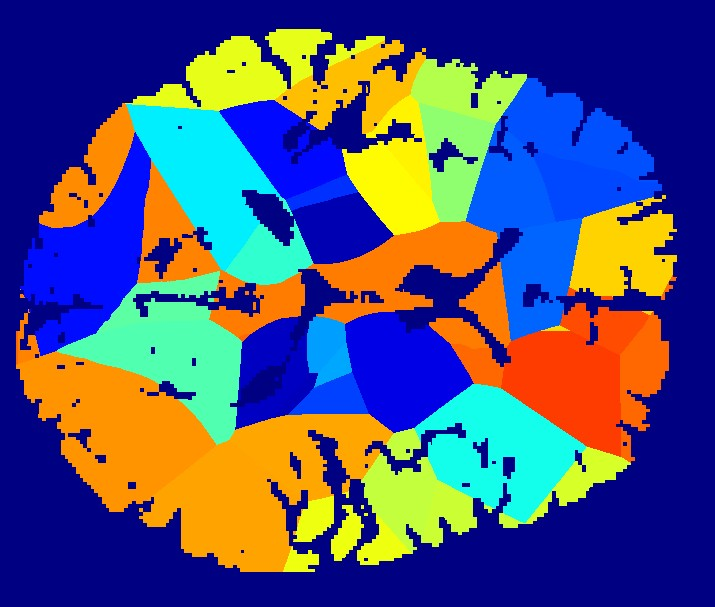
\includegraphics[width=9cm]{2_13_territoire_arteres_veines}
\caption{Illustration des territoires définit sur la base des couples artère-veine.}
\label{fig:2_13_territoire_arteres_veines}	
\end{figure}	
%%%
%%%
Dans une première étape, nous réalisons une segmentation sur la base de l’imagerie $T_1$ (voir Appendice~\ref{sec:pretrait}). Les volumes matière grise et blanche sont ainsi extraits et un masque de ces tissus créé (probabilité matière grise + blanche > 0.9). En associant à chaque voxel de ce masque le label correspondant au couple artère-veine le plus proche (voir fin du paragraphe~\ref{sect:graph_creation}), on reconstruit les territoires (Figure~\ref{fig:2_13_territoire_arteres_veines}). \\
Les volumes de ces territoires permettent grâces aux rapports issues de littérature d’estimer les volumes des compartiments : 
\begin{equation}
\label{eq:volumesac}
V_{c}\,=\,\bigl(V_{s}\, *\,d_{c-a}\bigr)\, *\,\frac{V_{Ref_{c}}}{V_{Ref_{c}}*V_{Ref_{a}}},
\end{equation}
avec $V_c$ et $V_a$  les volumes des capillaires et des artérioles, $V_s$ le volume segmenté, $d_{c-a}$ la densité estimée d'artérioles et de capillaires dans un volume (selon~\cite{Moody2004}), et les $V_{ref}$ associés étant les volumes moyens des compartiments issus de la littérature.\\
Pour les veinules, nous n’avons pas l’information de densité. Le volume est donc estimé sur la base des volumes capillaires et artériolaires précédemment trouvés en résolvant : 
\begin{equation}
\frac{V_{v}}{V_v\,+\,V_a\,+\,V_c}\,=\,\frac{V_{ref_{v}}}{V_{ref_{v}}\,+\,V_{ref_{a}}\,+\,V_{ref_{c}}},
\end{equation}
avec $V_a$ et $V_c$ les solutions de~\ref{eq:volumesac}, et les volumes de référence toujours donnés par la littérature.\\
De même la longueur totale entre artères et veines est subdivisée en trois longueurs (artérioles, capillaires, veinules) sur la base des proportions fournit par la littérature (\cite{Zagzoule1986}). En l’état, faute d’informations structurales complémentaires, nous n’utilisons pas de facteurs géométriques correctifs supplémentaires (de type dimensions fractales), pour tenir compte du caractère ramifié de cette partie de la structure. \\
A partir des volumes et des longueurs de chaque compartiment, les rayons sont déterminés simplement (Équation~\ref{eq:rayons}). \\
Les rayons moyens des différents compartiments peuvent être visualisés (Figure~\ref{fig:2_13_profil_rayons}) et leur différences relatives mis en comparaisons aux données de la littérature (par exemple dans le chapitre suivant figure~\ref{fig:4_3_zagzoule}). Par ailleurs, les données quantitative illustrées dans le Tableau~\ref{tab:tab_profil_rayons} montrent des longueurs du même ordre de grandeur (bien que souvent plus élevés dans le modèle de Zagzoule et al.). On voit ainsi que des artères aux veines, les proportions des caractéristiques des différents tubes sont comparables. En revanche l'écart est important en terme de nombres d'artères et de veines, ce qui s'explique par d'une part : le niveau de détails de notre segmentation et d'autres part le fait les données de Zagzoule et al. ne sont pas issues directement de données terrain, mais des estimations.\\
 La comparaison de nos mesures aux données de BraVa (voir Chapitre~\ref{sec:anat_art}) permet d'évaluer l'écart de notre modèle à des données similaires. Le résultat met en évidence un nombre inférieur de moitié en terme de branches de notre méthode en rapport de BraVa. Au vue de l'approche manuelle privilégiée par ce dernier ce résultat est cohérent. La longueur moyenne des segments en revanche est similaire, bien que des écarts peuvent exister du fait de l'écart précédement décrit. On notera par ailleurs que les longueurs sont plus faibles que celles initialement utilisées par Zagzoule et al.. Les informations sur les calibres des vaisseaux ne sont cependant pas disponibles. \\

%%%
\begin{table}
\caption{Caractéristiques de l'architecture selon différents modèles. Le nombre d'artérioles, capillaires et veinules de notre modèle regroupe un ensemble de vaisseaux d'un territoire.}
\label{tab:tab_profil_rayons}
\begin{tabular}[!t]{l|l l}
\centering
      & Zagzoule & Notre modèle  \\
\hline
   Artères : aire (cm²) & 3.41 (5.6 \%)&  6.24  (0.8 \%) \\
   Artères : longueur (cm) & 83 &  29 \\
   Artères : nombre & 3950 &  115 \\
   Artérioles : aire (cm²) & 4.74 (7.7 \%)&  27.2  (8.7 \%)\\
   Artérioles : longueur (cm) & 35 &  23.4 \\
   Artérioles : nombre & 35000 &  45 \\
   Capillaires : aire (cm²) & 38  (62.3 \%)&  217.8  (69.9 \%)\\
   Capillaires : longueur (cm) & 5.236 &  3.34 \\
   Capillaires : nombre & 202000 &  45 \\
   Veinules : aire (cm²) & 9.49 (15.5 \%)& 54.5 (17.5 \%)\\
   Veinules : longueur (cm) & 35 &  23 \\
   Veinules : nombre & 72000 &  45 \\
   Veines : aire (cm²) & 5.34  (8.76 \%)& 5.18 (3.12 \%)\\
   Veines : longueur (cm) & 78.5 &  26.5 \\
   Veines : nombre & 3896 &  24 \\
\hline

\end{tabular}
\end{table}
%%%
%%%
\begin{figure}[!t]
\centering
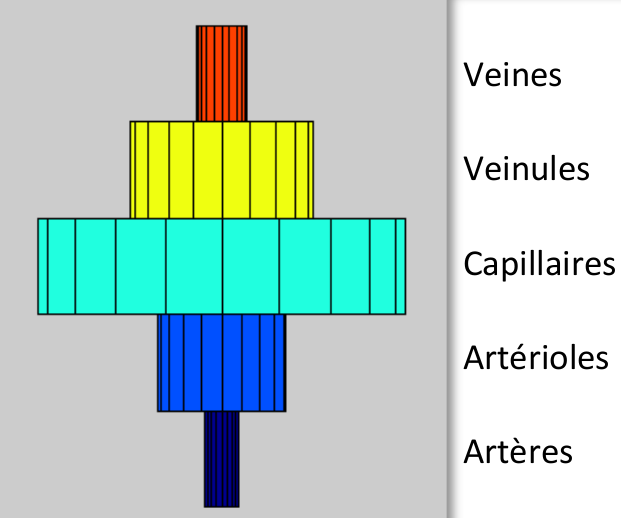
\includegraphics[width=10cm]{2_13_profil_rayons}
\caption{Illustration des rayons moyens dans les différents compartiments du système.}
\label{fig:2_13_profil_rayons}	
\end{figure}	

%%%
%%%
%%%
\section{Le système ventriculaire}
\label{sec:syst_ventr}
A ce stade, nous possédons une architecture complète allant des entrées artérielles aux veines. Il manque cependant les informations relatives à la circulation du liquide cérébro-spinal. Ce dernier peut être segmenté facilement via l’outil SPM (voir Appendice~\ref{sec:pretrait}). Cependant, cet outil ne fournit aucun moyen d’identification directe des différents ventricules. Une toolbox SPM nommée ALVIN pour « Automatic Lateral Ventricle delIneatioN » propose d’identifier sur la base d’une imagerie $T_1$, et de sa segmentation de données a-priori, les ventricules latéraux (\cite{Kempton2011}). Cependant afin de reproduire un système cohérent, nous souhaitons intégrer les ventricules latéraux, mais aussi les troisième et quatrième ventricules à notre description. Des outils plus ou moins sophistiqués existent par utilisation de modèles du système ventriculaires et d’algorithmes de croissance de région  (\cite{Liu2009},\cite{Schnack2001}) mais peu sont disponibles gratuitement pour la communauté. Or les ventricules peuvent être facilement segmentés manuellement en 4 clics via des outils de traçage semi-automatique de roi 3D basés sur les intensités. Un exemple est le « 3D painting tool » proposé par MRIcron (\cite{Rorden2007}). En effet, les ventricules apparaissent en hyposignaux clairement délimitable des autres tissus. MRIcron permet de sélectionner automatiquement tous les voxels dans un rayon donné ayant un faible écart en termes d’intensité à un voxel de référence. Des cycles successifs d’érosions/dilatations limite les risques que la ROI « bave » dans des régions non désirées. Cette méthodologie est simple à mettre en place, et efficace (figure ~\ref{fig:2_14_ventricules_segmentes}). \\
%%%
\begin{figure}[!t]
\centering
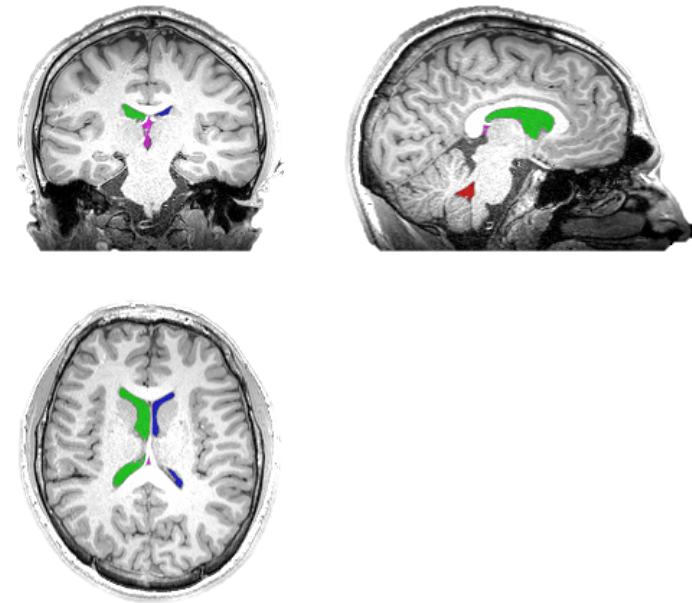
\includegraphics[width=10cm]{2_14_ventricules_segmentation}
\caption{Segmentation semi-automatique des ventricules par MRIcron sur une image T1. Chaque ventricule est identifié
par une couleur différente.}
\label{fig:2_14_ventricules_segmentes}	
\end{figure}	
Le choix se pose donc entre une approche automatique ayant un coût conséquent en termes
d’implémentation et une approche semi-automatique rapide. La deuxième solution, bien que
nécessitant une intervention de l’utilisateur a été privilégiée. En effet, bien que les algorithmes à
croissance de région puissent fournir des résultats intéressants, ils ne sont pas infaillibles. Or, la
manipulation réalisée sous MRIcron est simple, rapide, et assure une bonne qualité des résultats grâce
au contrôle utilisateur.\\
La description des volumes correspondant par des géométries cylindriques est imposée par la
logique de la construction de notre modèle, elle est peu conforme à la réalité structurale. Du point de
vue de l’élastance, en choisissant une longueur conventionnelle issue de la littérature (\cite{Linninger2009}), on peut
reporter de façon plausible les variations de volumes sur les variations de sections. Par contre le calcul
d’une résistance hydrodynamique entre ces longueurs (par une loi de poiseuille) n’est certainement
pas correct. Il est d’ailleurs vraisemblable qu’une partie importante de la résistance de ce système se
situe non pas dans les compartiments eux-mêmes, mais dans les conduits qui les relient. Néanmoins,
ce modèle simplifié maintient une description hydrodynamique semblable à celle des vaisseaux.
L’article de Linninger et al. (\cite{Linninger2009}) montre une bonne capacité de cette technique à reproduire des
phénomènes spécifiques à la circulation céphalo-rachidienne (hydrocéphalie).\\
On peut se réserver un paramètre d’ajustement de la résistance hydrodynamique des
compartiments du LCS qui multiplient la simple loi de Poiseuille et dont on pourra rechercher la valeur
la plus adéquate.
%%%
%%%
%%%
\section{Finalisation}
\label{sec:finalisation}
Le système est alors complet, chaque compartiment est représenté et décrit à travers son volume,
son rayon, et sa longueur. Dans la perspective d’une modélisation par un système d’équations
différentielles ordinaires, la structure peut s’avérer complexe à appréhender. En effet, nous allons
avoir des centaines de segments à modéliser, et les équations correspondantes devront être générées
automatiquement à partir de la description structurale. De ce fait, les situations telles que les
convergences de plus de trois vaisseaux peuvent complexifier l’implémentation d’un algorithme
générique de définition des équations. Une dernière étape de finalisation vise donc à :
%%%
\begin{figure}[!t]
\centering
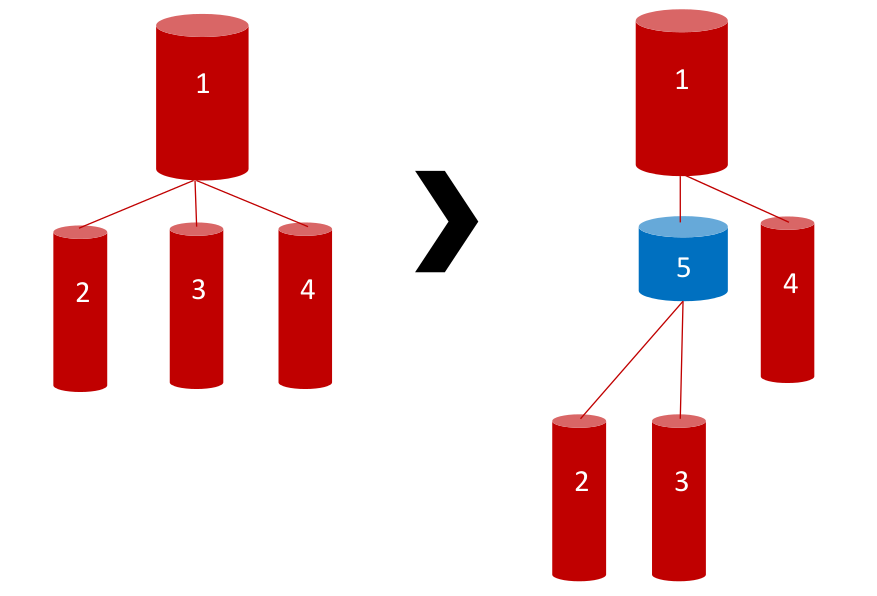
\includegraphics[width=14cm]{2_15_conversion_y}
\caption{Illustration de la conversion des vaisseaux à connexions multiples en connexions en Y. Les tubes représentent des
segments de vaisseaux, ils sont identifiés par un numéro. La conversion en connexions 2 vers 1 ou 1 vers 2 est réalisée par
l’insertion d’un nouveau tube (en bleu) de très faible longueur et de rayon identique au tube parent.
}
\label{fig:2_15_conversion_y}	
\end{figure}	
\begin{itemize}
\item Réduire les connexions entre les tubes à des connexions en Y (deux tubes vers un ou
l’inverse) : détails en Figure ~\ref{fig:2_15_conversion_y};
\item éliminer les boucles qu’il peut rester (hors polygone de Willis): en parcourant l’arborescence
et en ne conservant que les chemins les plus courts (ou le chemin suivant les vaisseaux les
plus gros de façon à maximiser les volumes) amenant d’une entrée aux branches terminales
des artères, ou d’une veine à la sortie.
\end{itemize}
Comme on le verra l’architecture ainsi finalisée pourra être importée dans le modèle et implémentée.


\bibliography{jeremythesebib}{}
\bibliographystyle{francaissc}